\documentclass{report}
\usepackage{fixlatvian}
\usepackage{graphicx}
\usepackage{verbatim}
\usepackage{geometry}
\geometry{top=30mm}
\usepackage[european]{circuitikz}
\usepackage{pgfplots}
\usepackage[backend=biber]{biblatex}
\addbibresource{Ye.bib}



\title{Vienkāršuelektrisku shēmu modelēšana}
\author{Roberts Oskars Komarovskis - REBMO2}
\date{09.03.2018}

\begin{document}




\maketitle

\chapter{Teorētiskā daļa}
\section{Ķēdes aprēķins}

\par1. Laboratorijas darbā 1.1 sadaļā tika veikts teorētiskais aprēķins, kur ar dotajiem lielumiem jāizrēķina sprieguma kritums uz diviem rezistoriem, kuri saslēgti virknē, izmantojot Oma likumu.  Visi aprēķinu lielumi ir apskatāmi \ref{tab_1} tabulā.
\\
\\
\\
\begin{equation}
R=\frac{U}{I}
\end{equation}
\begin{equation}
U=R*I
\end{equation}
\\
\\
\\
Oma likuma skaidrojums angļu valodā ņemts no mājaslapas \cite{ohmlik}\\\\
\cite[The potential difference (voltage) across an ideal conductor is proportional to the current through it. The constant of proportionality is called the "resistance", R. Ohm's Law is given by: V = I R where V is the potential difference between two points which include a resistance R.]{ohmlik}
\\
\\
\\
Oma likuma skaidrojums latviešu valodā ņemts no mājaslapas \cite{ohmliklv}\\\\
\cite[Oma likums nosaka sakarību starp spriegumu un strāvu elektriskās ķēdes posmā. Strāvas stiprums ir tieši proporcionāls spriegumam. Cik reizes izmaina spriegumu, tikpat reižu izmainās strāvas stiprums. Strāvas stiprums I ir atkarīgs arī no patērētāja elektriskās pretestības. Jo lielāka ir pretestība, jo mazāka strāva plūst vadītājā. Strāvas stiprums ir apgriezti proporcionāls elektriskajai pretestībai. Likums nosaukts par godu vācu fiziķim Georgam Simonam Omam (Ohm).]{ohmliklv}
\\
\\
\\
 Funkcijas $U_{R2}=f(R_2)$ līkne ir redzama attēlā \ref{diag_1}
\begin{table}
    \centering
    \begin{tabular}{|l|l|p{20cm}|}
    \hline
    R1 & 6 Ohm \\ \hline
    R2 & 9 Ohm \\ \hline
    V1 & 15,7V \\ \hline
    UR1 & 6,276V \\ \hline
    UR2 & 9,414V \\ \hline
    \hline
    \end{tabular}
    \caption{Aprēķinu lielumi}
    \label{tab_1}
\end{table}
\begin{figure}
\centering
\begin{circuitikz}
    \draw (0,0)
    to node[ground]{}(0,-1)
    to [battery1,V=15.7V](0,3)
    to [resistor, R=6 $\Omega$](4,3)
    to [resistor, R=9 $\Omega$](4,0)
    to node[ground]{}(4,-1);
\end{circuitikz}
\label{sch_1}
\caption{Latexā iegūtā shēma}
\end{figure}
\begin{figure}

\centering
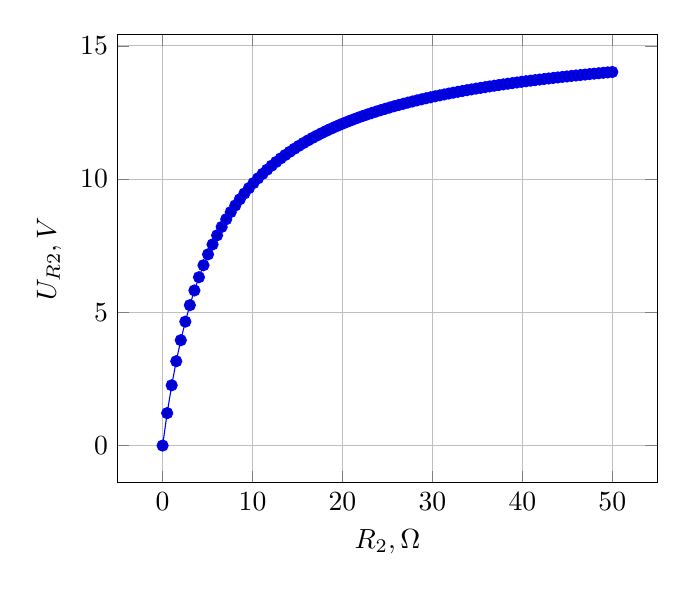
\begin{tikzpicture}
	\begin{axis}[
	    domain=0:50, 
        samples=100, 
        color=black,
		xlabel={$R_2 ,\Omega$},
		ylabel={$U_{R2}, V$},
		grid
	]
	% use TeX as calculator:
	\addplot {(15.7*x)/(6+x};
	\end{axis}
\end{tikzpicture}
\caption{Teorētiskā diagramma}
\label{diag_1}

\end{figure}



\chapter{Praktiskā daļa}
\section{Darbs ar GEDA programmām}

\subsection{Darbs ar gschem}

Iegūtā shēma, kas tika iegūta ar gschem ir redzema \ref{att1}
\begin{figure}[h]
    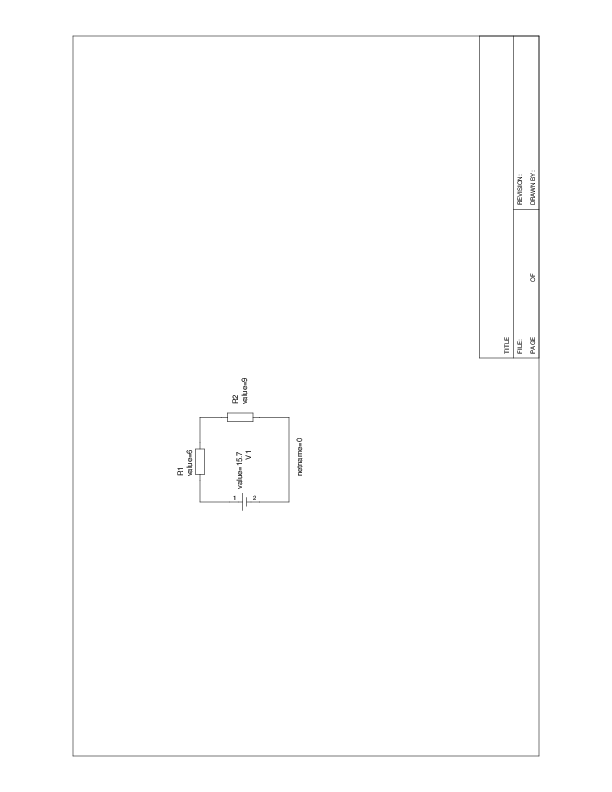
\includegraphics[scale=0.5, angle=-90]{01.png}
    \caption{gschem shema}
    \label{att1}
\end{figure}


\subsection{Darbs ar gnetlist}
\begin{verbatim}


* Spice netlister for gnetlist
R1 1 2 6
R2 2 0 9
V1 1 0 15.7
.END
\end{verbatim}


\subsection{Darbs ar ngspice}
\begin{verbatim}
\end{verbatim}\\
\ref{att2} redzams spriegums pirmajā mezglā pirms R1\\\\
\ref{att3} redzams spriegums otrajā mezglā pirms R2\\

\begin{figure}[h]
    \centering
    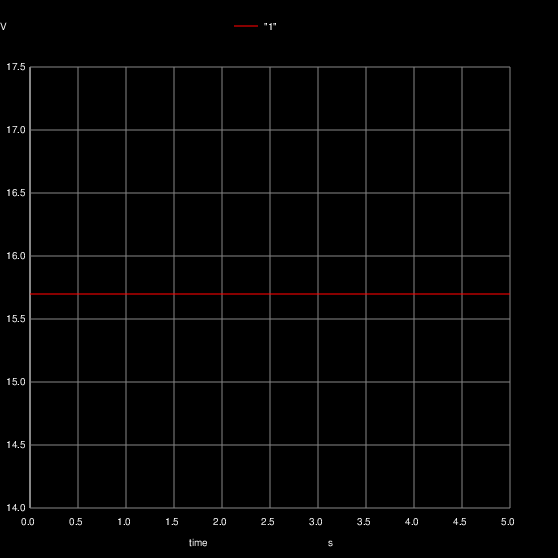
\includegraphics[scale=0.3]{011.png}
    \caption{Spriegums pirmajā mezglā}
    \label{att2}
\end{figure}


\begin{figure}[h]
    \centering
    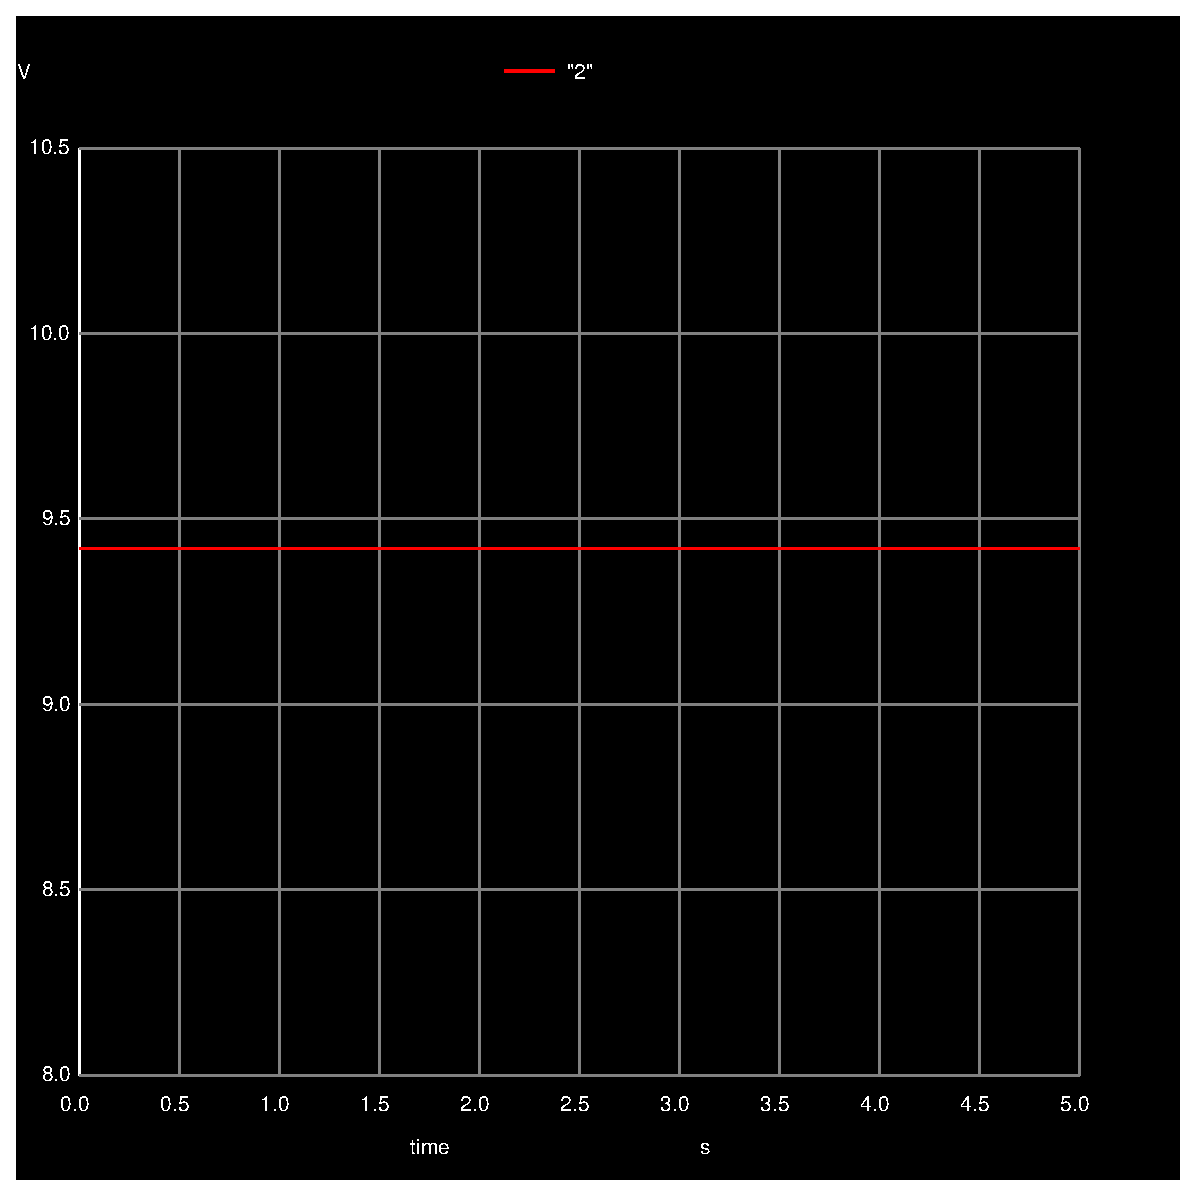
\includegraphics[scale=0.3]{012.ps}
    \caption{Spriegums otrajā mezglā}
    \label{att3}
\end{figure}
\section{Darbs ar QUCS programmām}
\begin{verbatim}
\end{verbatim}
\ref{att4} attēlā redzama shēma, kura tika izgatavota ar qucs programmu.
\begin{figure}[!b]
    \centering
    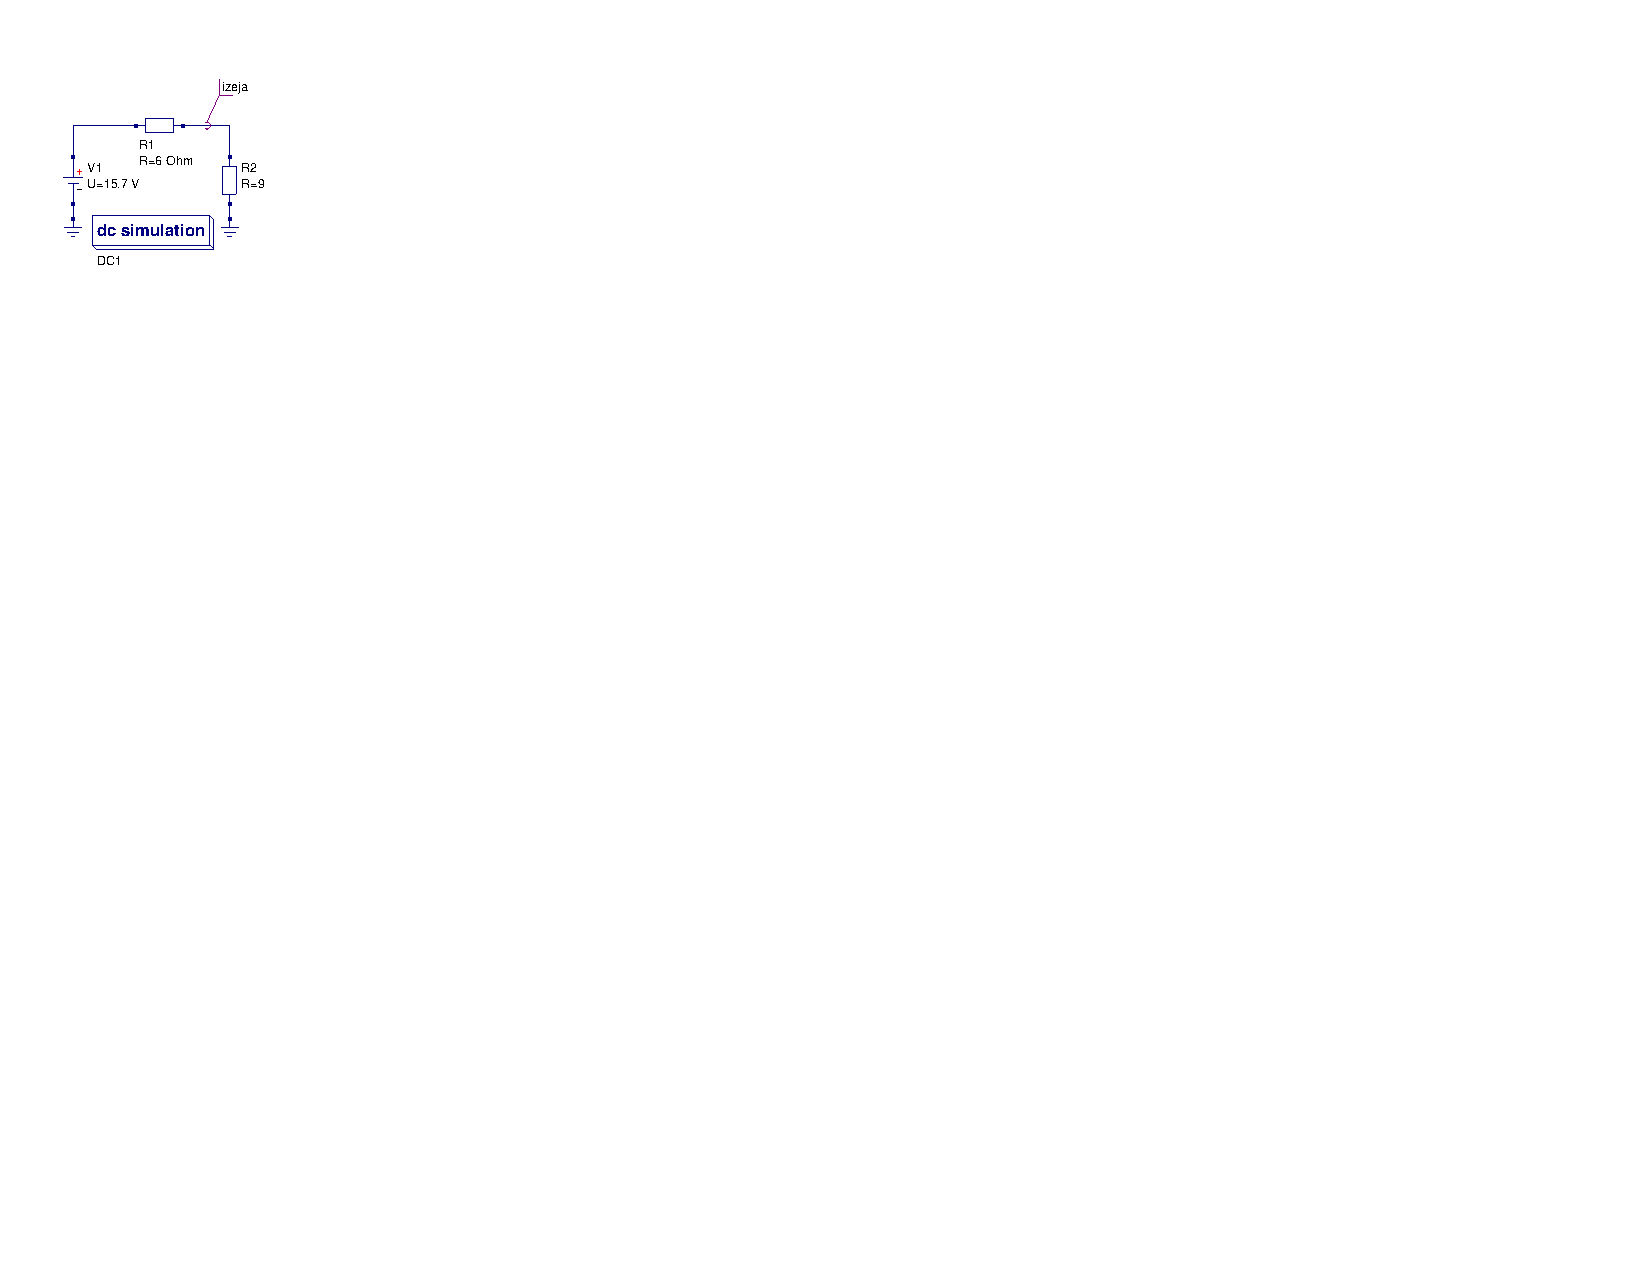
\includegraphics[scale=1.5, angle=270]{qucsscheme.pdf}
    \caption{Shēma, kas tika iegūta ar QUCS}
    \label{att4}
\end{figure}
\begin{verbatim}
    
    
\end{verbatim}
    
    Ar QUCS komponenti "Parameter Sweep" tika iegūta simulācija, kuras laikā R2 mainījās no 5 Ohm līdz 50 Ohm ar soli 5 Ohm. \ref{att5} redzams grafiskais attēlojums R2 vērtībām simulācijas laikā, kā arī tabula, kas attēlo R2 skaitliskās vērtības. Arī šāda tabulācija un grafiku zīmēšana ir iespējama izmantojot QUCS
    
\begin{figure}[!b]
    \centering
    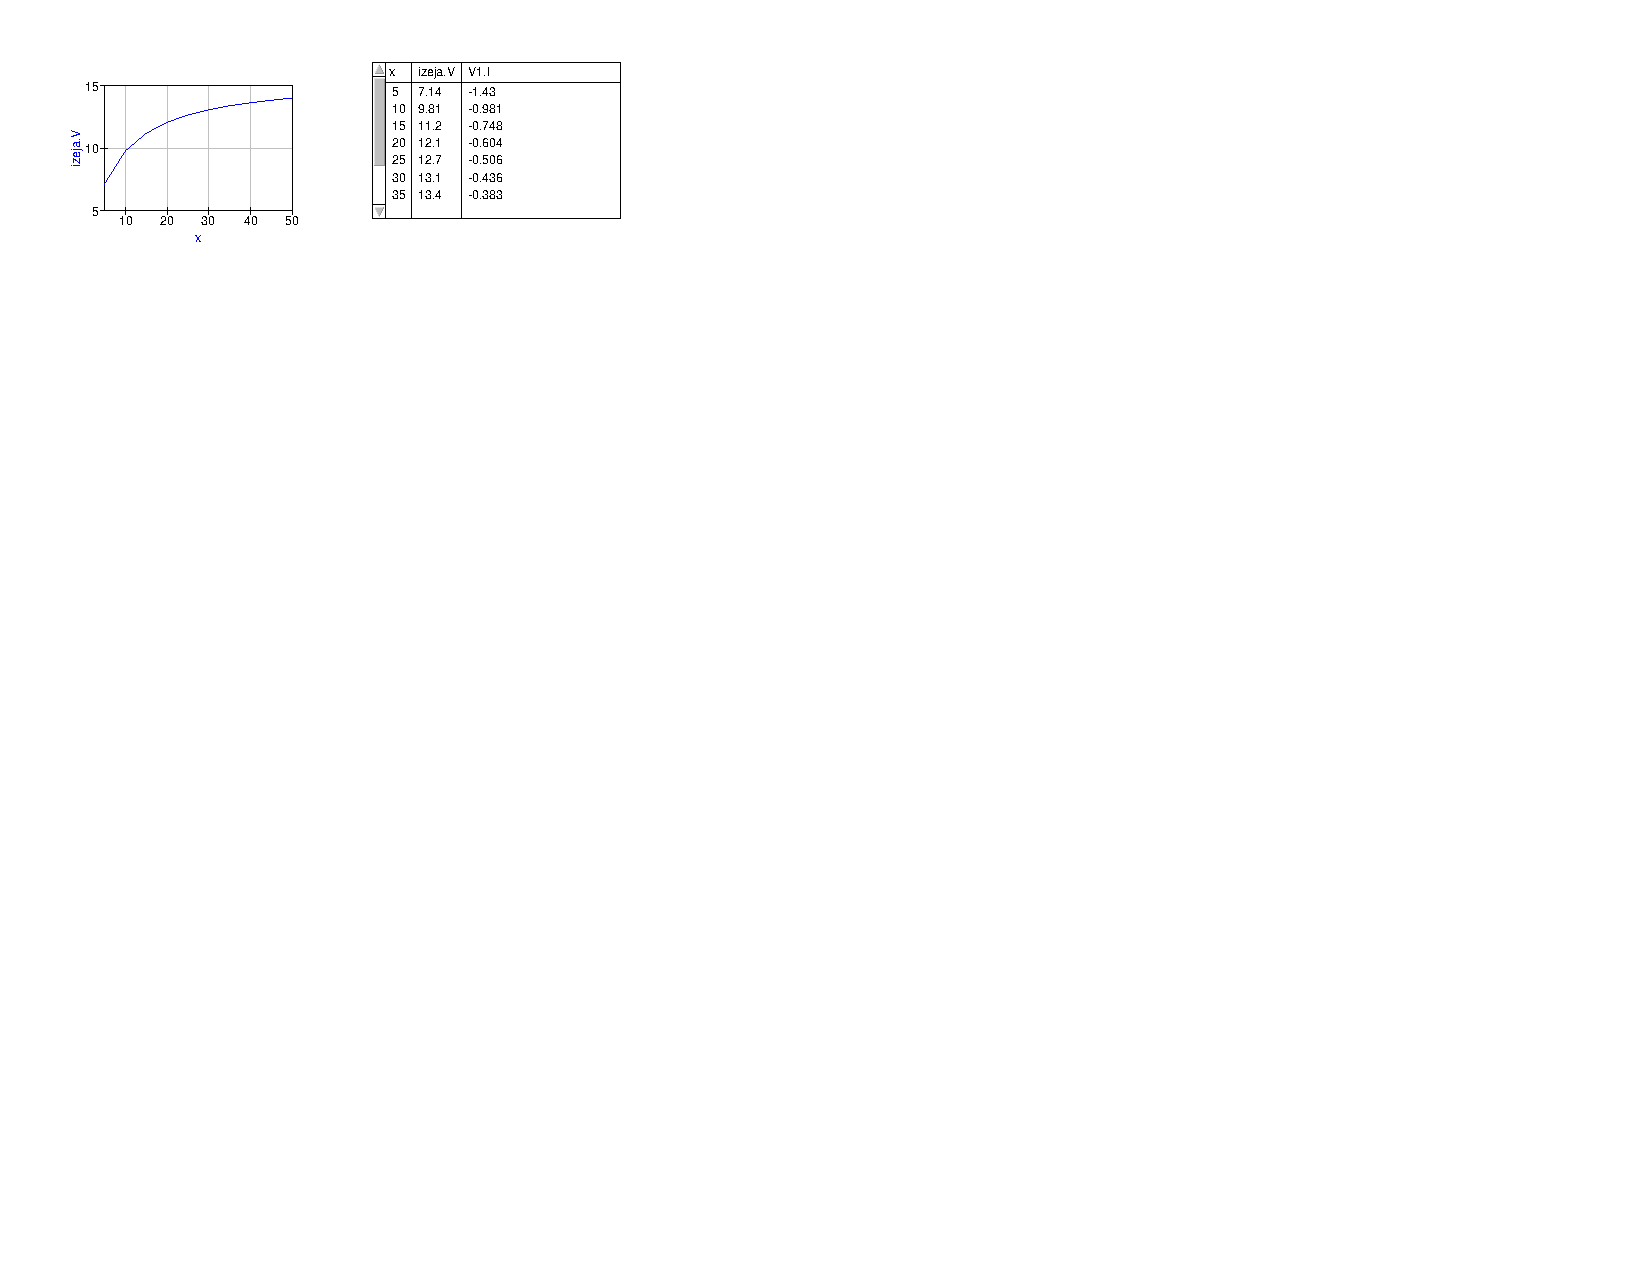
\includegraphics[scale=1.5,angle=270]{qucssweep.pdf}
    \caption{Parameter sweep rezultāti}
    \label{att5}
\end{figure}

\printbibliography

\end{document}
